
\section{Case Study}

Our case study is divided into two sections. In the first, we focus on understanding how countries cluster in thematic space, particularly with respect to protest. In the second, we consider in greater detail how patterns in the protest theme differentiated by media provide support for claims explored by \cite{cottle_media_2011}.

\subsection{Connecting countries and themes}

\begin{figure*}[th]
	\centering
	\begin{tabular}{cc}
		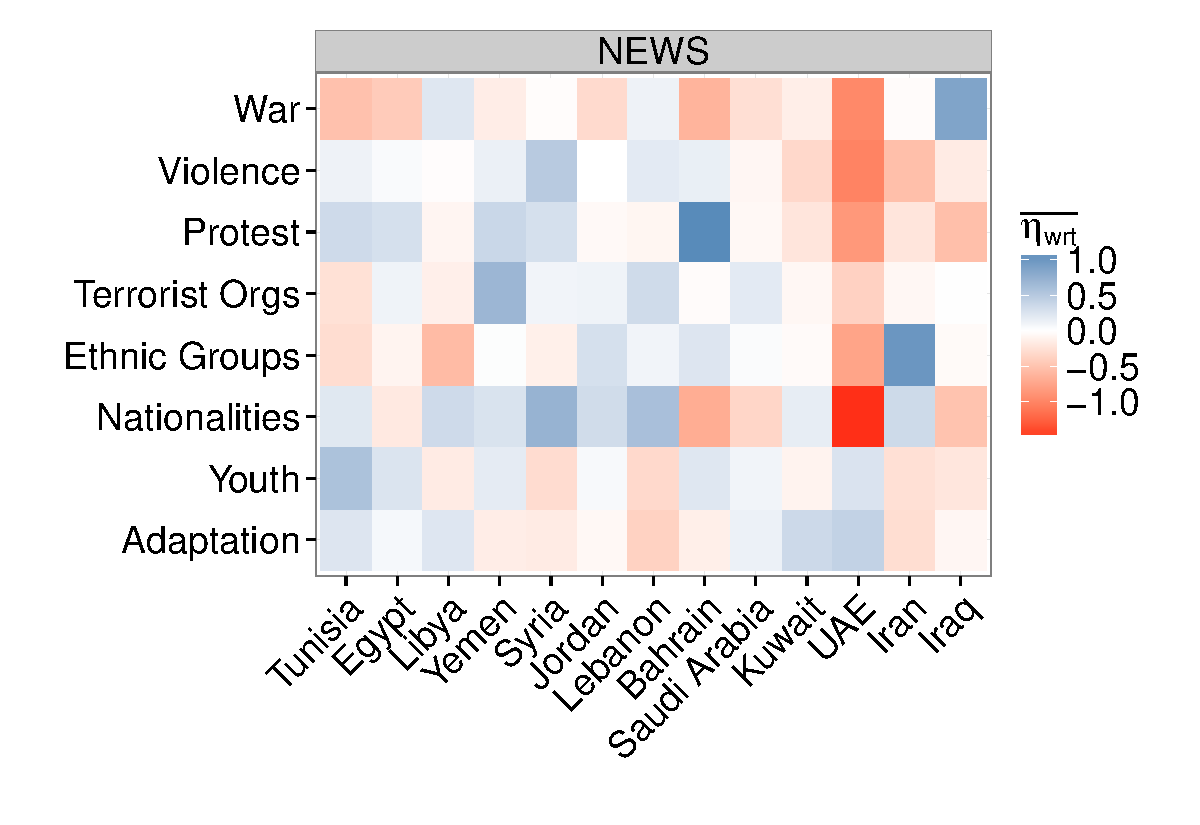
\includegraphics[width=.5\textwidth]{imgs/activity_topics_news} &
		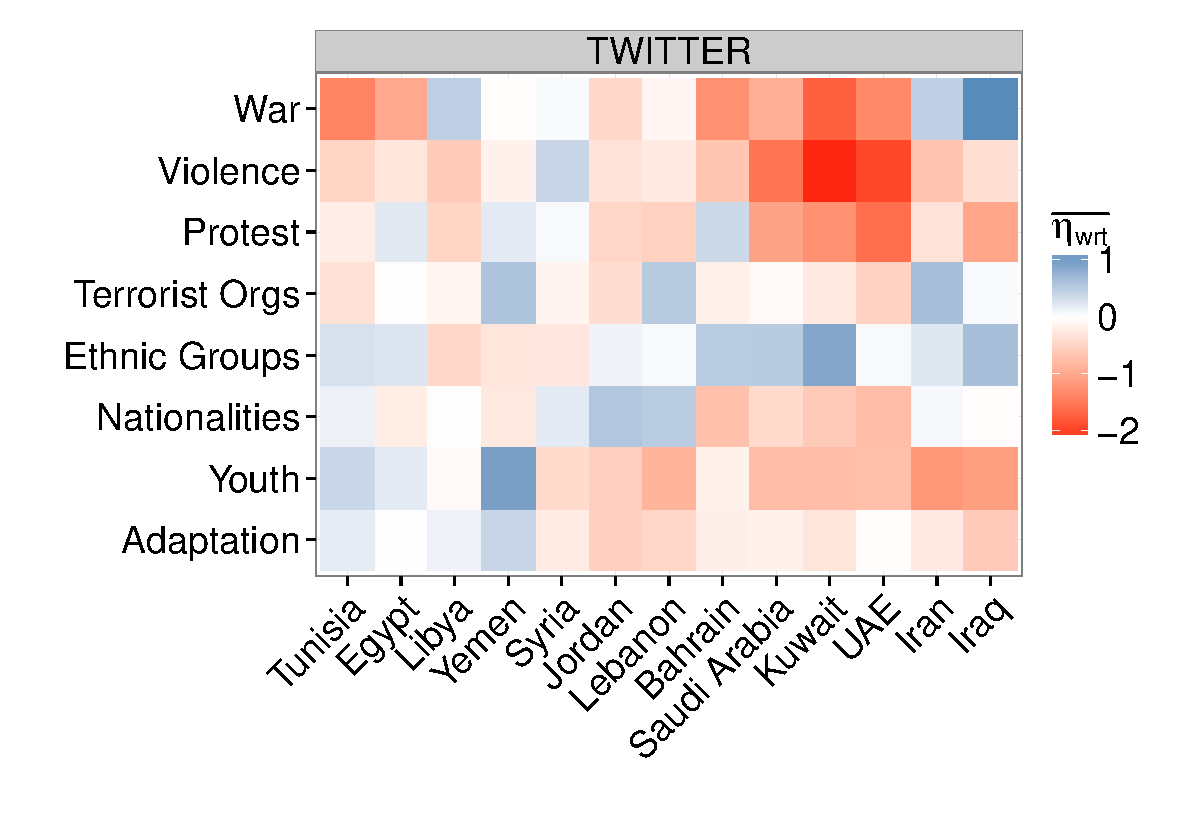
\includegraphics[width=.5\textwidth]{imgs/activity_topics_twitter} \\
	\end{tabular}
	\caption{Mean activation rate over all months for each country and category combination.  The higher the value above 0, the darker the blue. The lower the value below 0, the darker the red. }
	\label{fig:overall}
\end{figure*}


Figure \ref{fig:overall} shows two plots, one for news (left) and one for Twitter (right). Each plot depicts a heatmap of the mean activation values ($\overline{\eta_{w,r,t}}$) over all months for each country/theme combination. The higher the mean activation score above zero for a particular theme/country combination, the darker blue the square. The lower the value below zero, the darker the red. Additionally, note that values are interpretable relative to global activity of each topic/country combination. That is, the dark blue square in the top right of the Twitter plot shows that, on average, relative to other countries, discussions of war were more frequent in Iraq than the discussion of other topics. 

Figure \ref{fig:overall} suggests two fascinating patterns in how countries clustered along themes explored here. First, we considered how countries clustered along perhaps the most interesting theme with respect to the Arab Spring, that of protest.  Figure~\ref{fig:overall} shows that for countries in which protests occurred at relatively low levels (Iran, Iraq, Saudi Arabia and the UAE), discussion of protests were low in both the news and Twitter data. Interestingly,  however, even in countries where relatively high levels of protest occurred, a distinction can be made in the level of discussion of protest between countries where revolutions are still ongoing or succeeded in overthrowing the government (Egypt, Yemen, Tunisia, Libya, Bahrain and Syria) versus those where little social change occurred (Jordan, Kuwait, Lebanon).  In all but Libya, countries where social change followed protests showed positive (above zero, on average) levels of discussion about protest in the news media data. In contrast, countries where protests failed to produce significant results showed negative activation rates for this theme, on average, across time.  In the Twitter data the same patterns hold, although discussion of protest in Tunisia, who's government fell before the beginning of our data collection, is also negative.

\begin{figure}[t]
	\centering
	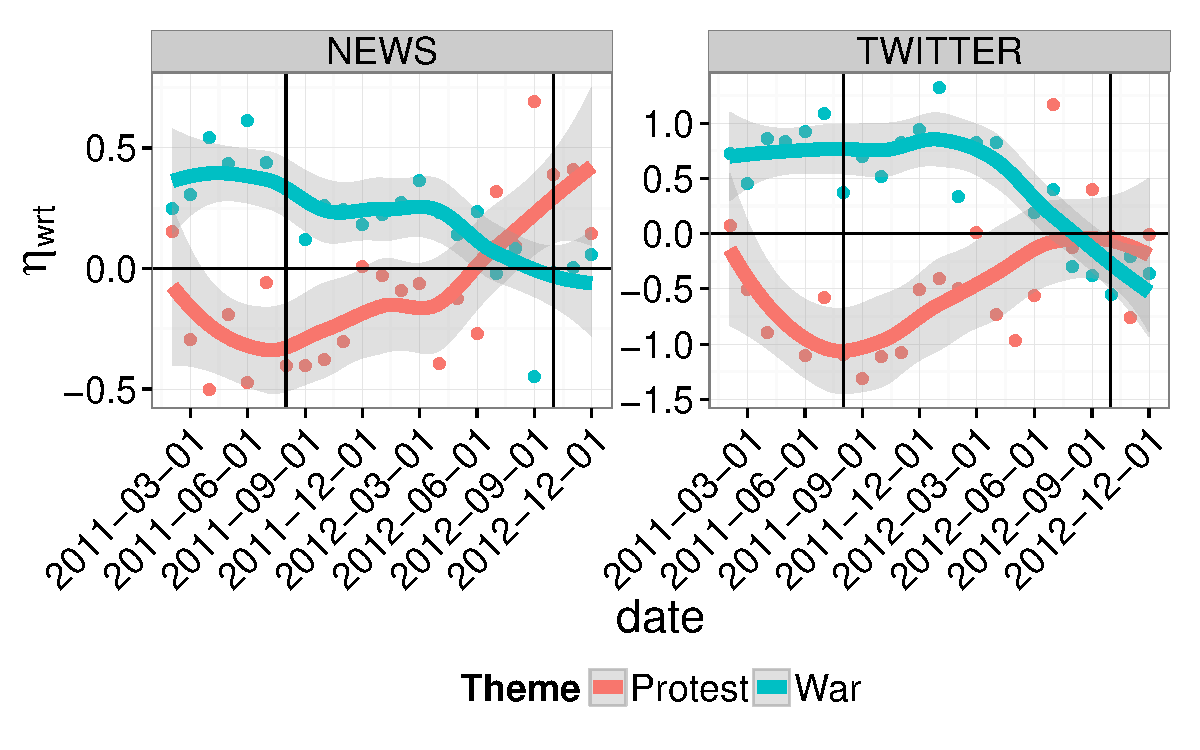
\includegraphics[width=.5\textwidth]{imgs/lib_protest_viol}
	\caption{Relationship between the protest and war themes over time in Libya. Points represent estimates from the model, nonparametric smoothed estimates with 95\% confidence intervals are provided as lines to ease visual observation of trends.}
	\label{fig:prot_viol}
\end{figure}

In sum, results show that in both Twitter and news media, levels of discussions about protest clustered into countries in which important social change occurred during the period, where positive activation scores for protest were observed, and countries where little or no social change occurred, where negative activation scores were seen. The lone exception to this categorization was Libya, where a six month civil war eventually led to the downfall of the ruling regime. We can understand why low levels of discussion on the subject of protest occurred by looking at the way in which protest was discussed over time in Libya. Figure~\ref{fig:prot_viol} shows the activation rates of the categories protest and war over time in Libya. The first vertical black line represents, approximately, the point at which the ruling regime was overthrown, the second black line represents the attack on the U.S. consulate in Benghazi.  As we can see, the focus in Libya on protest may largely have been mediated by a focus on the civil war and its aftermath.  However, as unrest grew again in the face of complaints about the new regime, we do see a renewed trend towards protest, which could be seen as an initial indicator of a return to civil unrest.  This intricate relationship between discussions of war and protest is of particular interest in understanding how unrest leads to organized violence.
 
\begin{figure}[t]
	\centering
	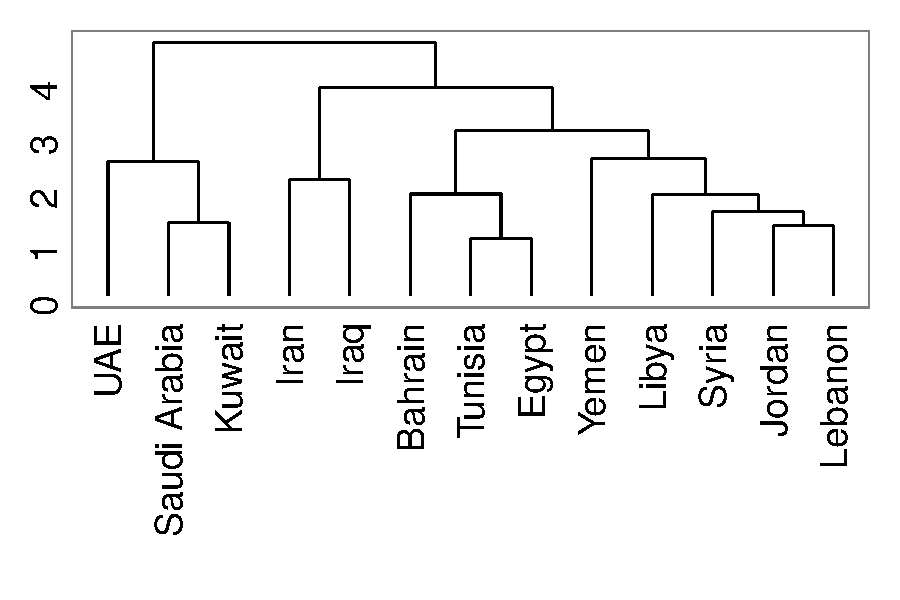
\includegraphics[width=.5\textwidth]{imgs/country_dendro}
	\caption{Hierarchical clustering of our 13 countries based on mean activation levels across all categories for both news and Twitter }
	\label{fig:clust}
\end{figure}

Figure~\ref{fig:overall} also suggests there exists clusters of countries that exist at a larger level than simply distinctions across protests.  To better evaluate the extent to which this clustering exists, we perform a standard, complete-linkage, agglomorative clustering, where each country is represented by sixteen features (the eight categories shown in Figure~\ref{fig:overall} for both news and Twitter). Figure~\ref{fig:clust} presents a dendrogram of the resulting clustering.  Figure~\ref{fig:clust} shows that the oil-rich nations of Saudi Arabia, Kuwait and UAE, where little social change occurred, showed similar thematic structures.   Similarly, nations with which the United States has the strongest tensions, Iran and Iraq, cluster together.  Figure~\ref{fig:clust} shows that these five countries  are heavily separated in thematic content from nations where social change occurred, although they are also separated from perhaps the more similar nations of Lebanon and Jordan.  Within the cluster holding nations where large-scale social change occurred, we observe that Tunisia and Egypt are the most tightly connected, an indication of the extent to which these two revolutions were tied together. 

\subsection{Temporal patterns in protests}

\begin{figure}[t]
	\centering
	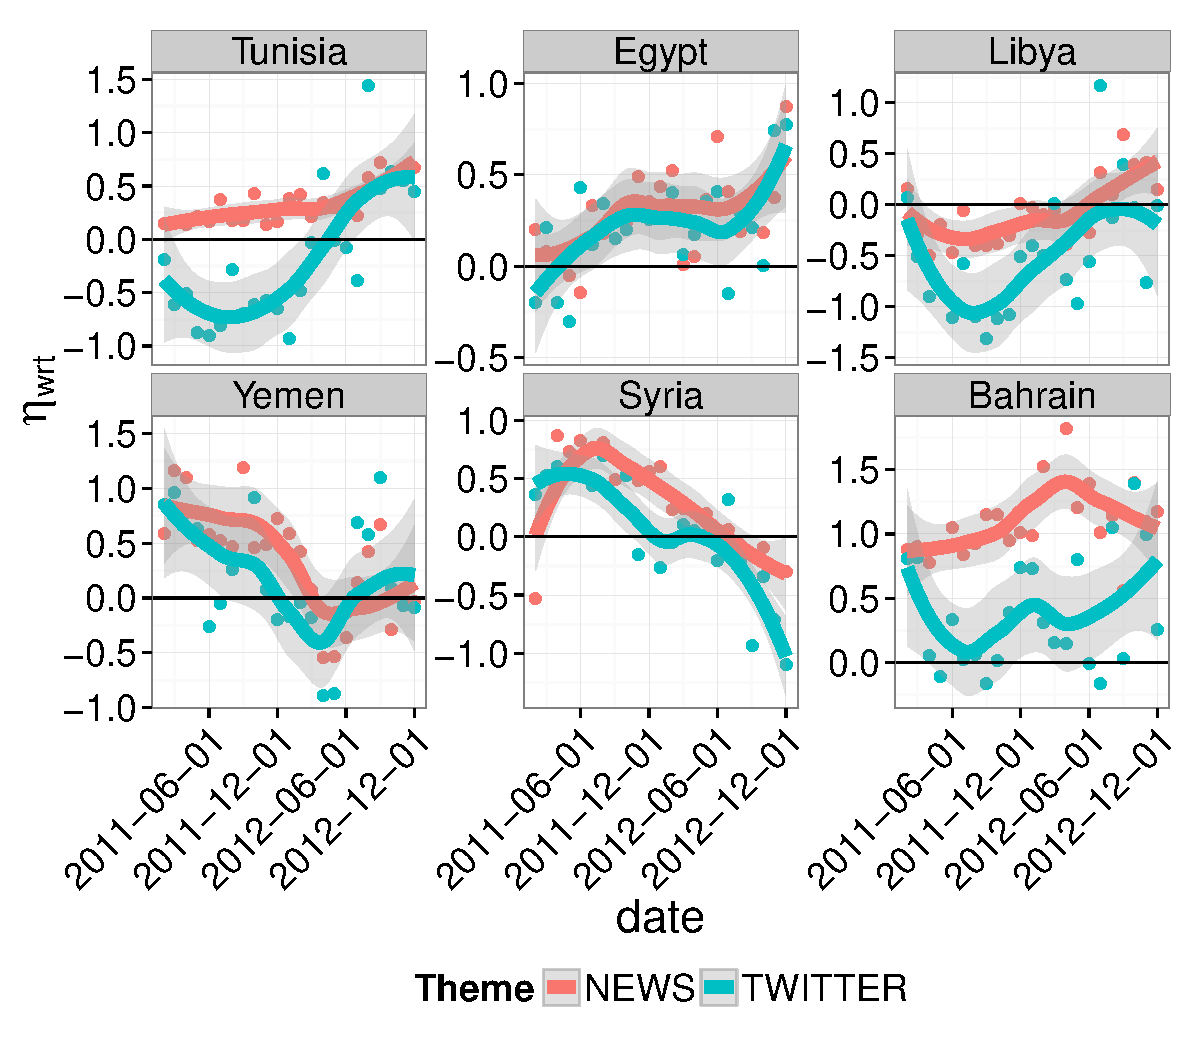
\includegraphics[width=.5\textwidth]{imgs/cottle}
	\caption{Activation Rates of protest over time for six countries of interest.  Points represent estimates from the model, nonparametric smoothed estimates with 95\% confidence intervals are provided as lines to ease visual observation of trends.}
	\label{fig:cottle4}
\end{figure}

Having noted that important clustering appears in average levels of activation with respect to protests, we turn now to how temporal patterns of protest played out in both news and Twitter for nations where high levels of social change occurred. Figure~\ref{fig:cottle4} illustrates activation rates for the theme of protest in news media and Twitter for Bahrain, Egypt, Libya, Syria, Tunisia and Yemen. Our findings, even over time, are consistent with the idea presented by \cite{cottle_media_2011} that new media played an important role in discussions of protests during the Arab Spring.  Perhaps more interestingly, \cite{cottle_media_2011} also argues that the relationship between social media and news media facilitated international recognition and protest legitimization, and provided human rights surveillance.  Our analysis is consistent with this assertion.  In contrasting results for Egypt, with its partially free press, to more restricted countries like Syria, Tunisia, and Bahrain, we observe that states with more oppressive regimes tend to show less of a relationship between social and news media. However, even in the more oppressive regimes, uptakes in Twitter activation with respect to protest always lead to corresponding changes in news activation rates which implies a strong interaction between the two media types. This relationship between news media and social media activation rates reinforce \citeapos{cottle_media_2011} premises. 

Since these clusters of countries we extract in this section are based on both news and Twitter, they cannot be attributed to just a western view of similarity among the countries.  Rather, they reflect some underlying commonality in the way information about and from the these countries is presented across a diverse media landscape.  On the one hand, these clusters show which countries have a common media profile and so, to an extent, a common pattern of media usage by the population.  On the other hand, these clusters may indicate how countries might be similarly influenced by a media campaign.  

%we pr little quantitative research exists analyzing the interaction between news and social media throughout the Arab Spring.   \citet{cottle_media_2011} presents the most comprehensive study to date and presents well argued hypotheses pertaining to the complex interactions between the two types of media and their implications for social change in MENA.  However, he does so with little empirical evidence and calls for ``careful documentation and comparative analysis in the months and years ahead.''  The following section will highlight how activation rates support or refute several of his assertions. 

%\todo{develop fig:cottle4. Decription: topic: protest countries: Bahrain, Egypt, Libya, Syria, Tunisia, Yemen. That depicts smoothed activation rates over time.  Similar to the blah2 plots}

% \todo{ I was not able to show a relationship between news v twitter correlation with either freedom of the press index or internet saturation.  I think there are a couple observations making this problematic.  First, very small set.  Protest and violence are only relatively important topics in a few countries, and not all of them are of equal interest in english speaking news media. I'm open to suggestions}


%	
%	\begin{figure*}
%		\centering
%		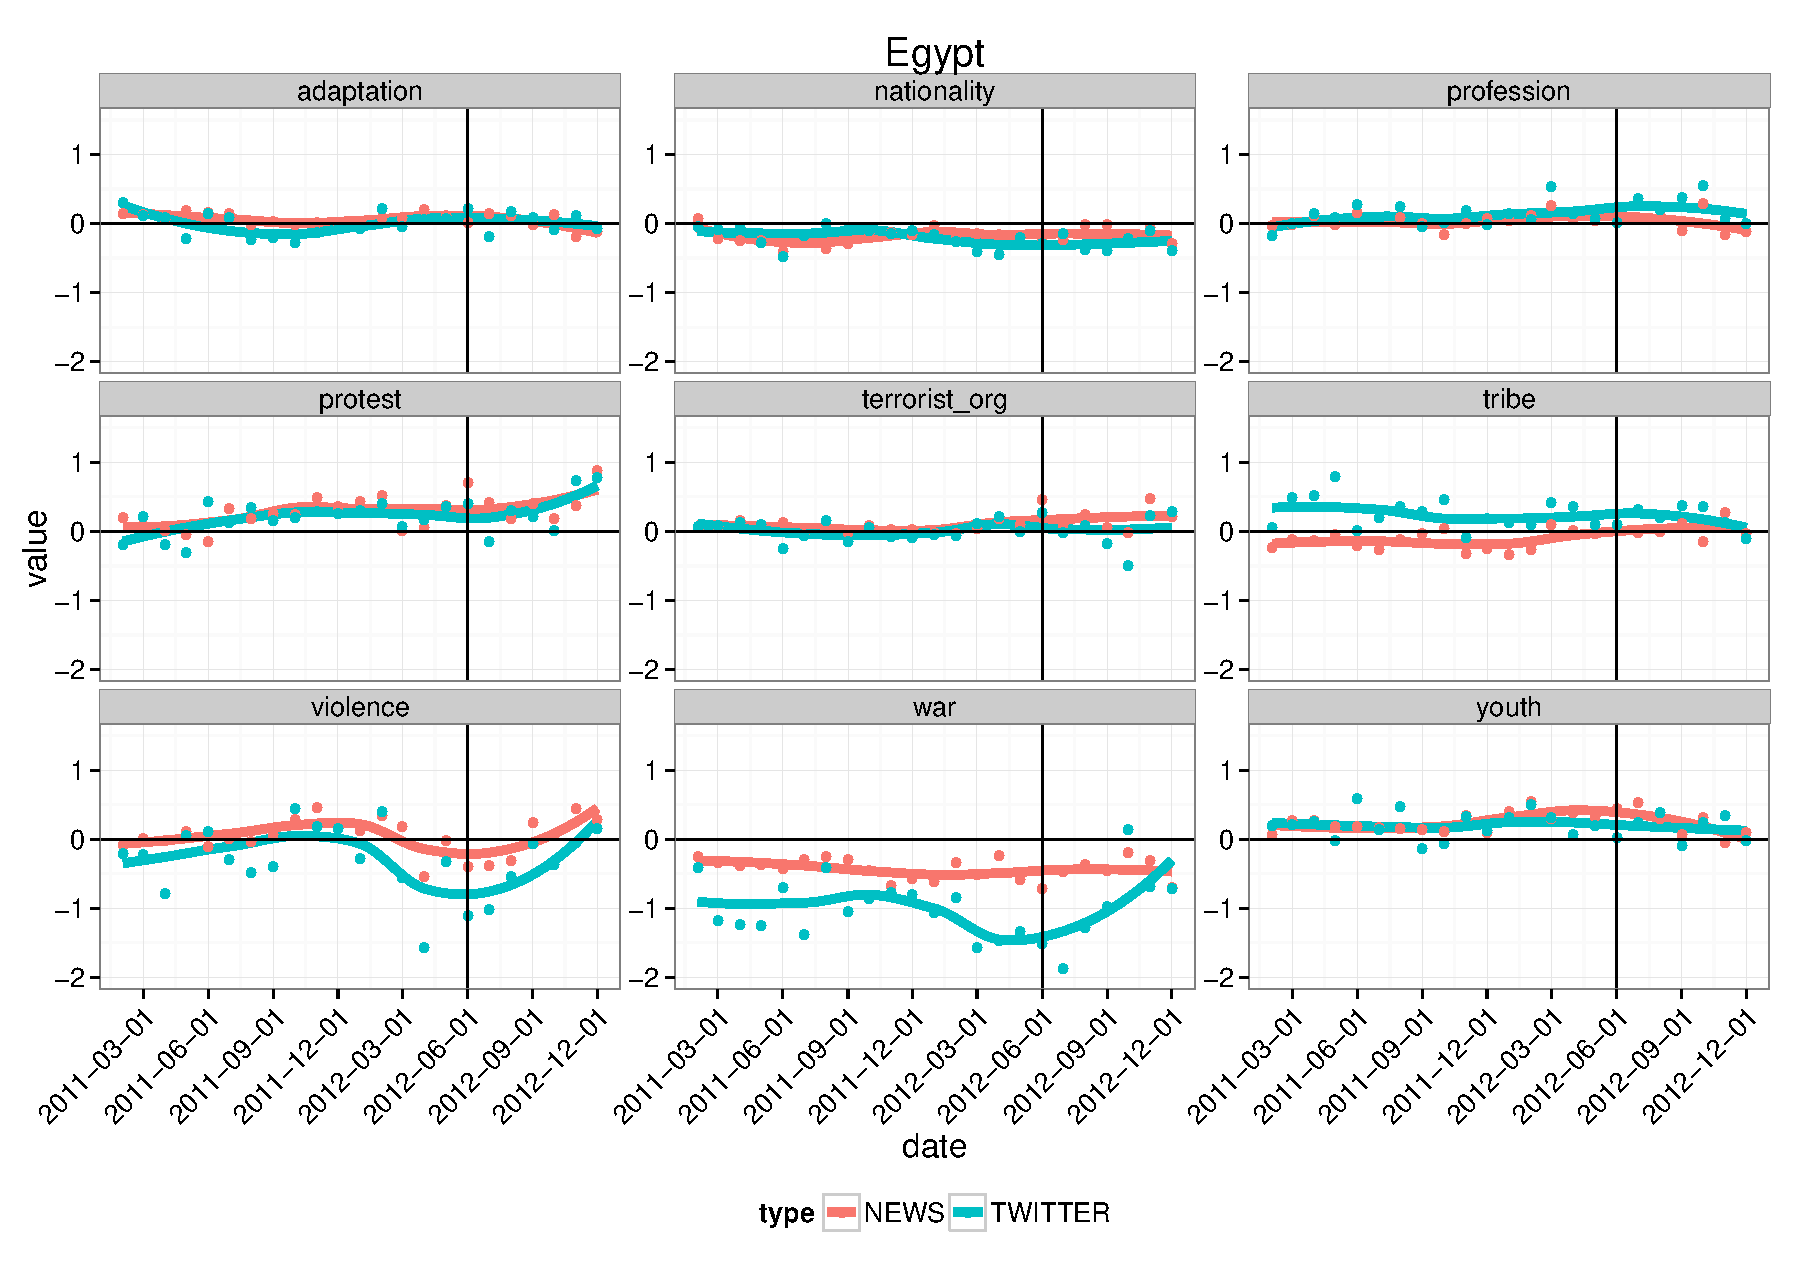
\includegraphics[width=\textwidth]{imgs/egypt.pdf}
%		\caption{Egypt: Black line is when Morsi is elected}
%		\label{fig:egypt}
%	\end{figure*}
%	
%	\begin{figure*}
%		\centering
%		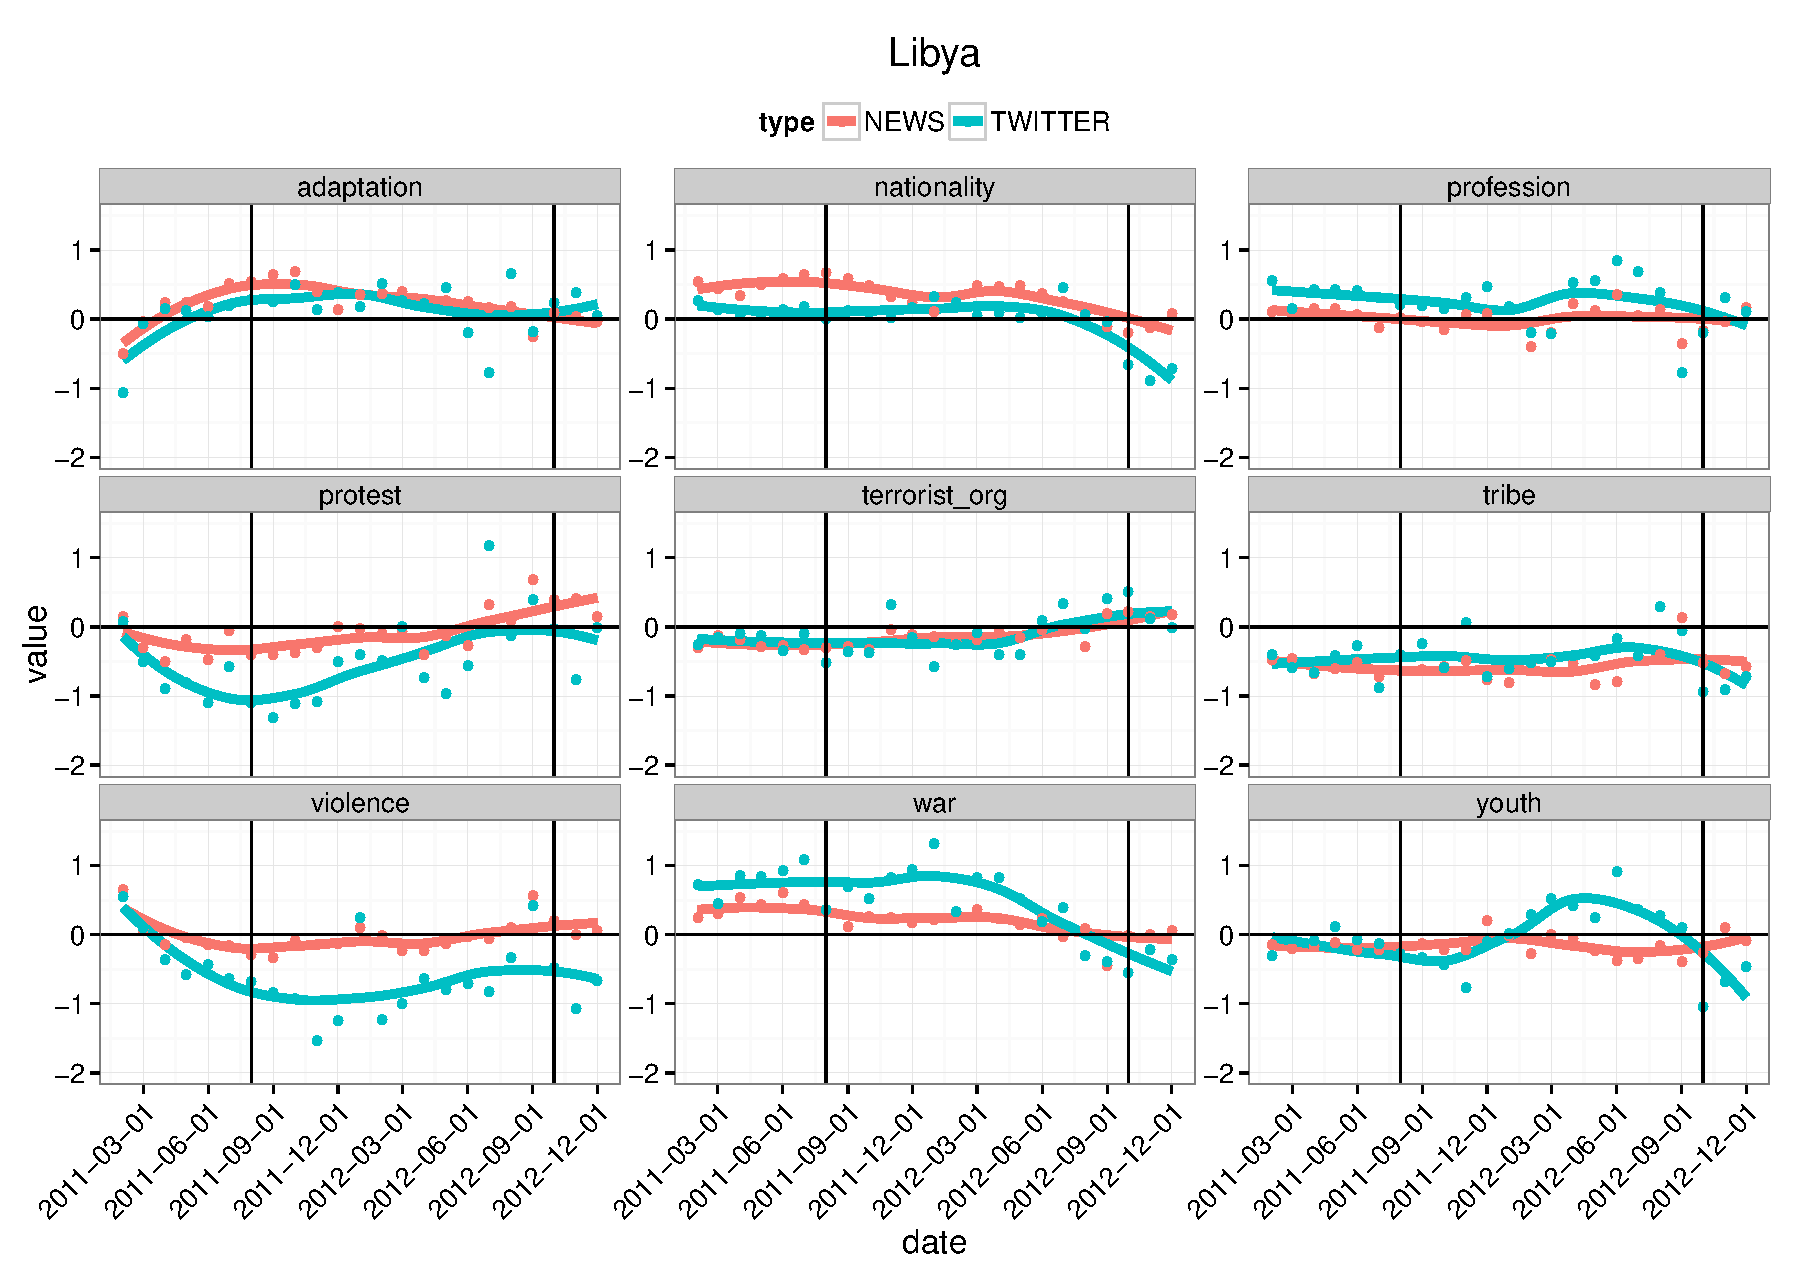
\includegraphics[width=\textwidth]{imgs/libya.pdf}
%		\caption{Libya: Black lines are death of Gaddafi and Benghazi }
%		\label{fig:libya}
%	\end{figure*}
%	
%	\begin{figure*}
%		\centering
%		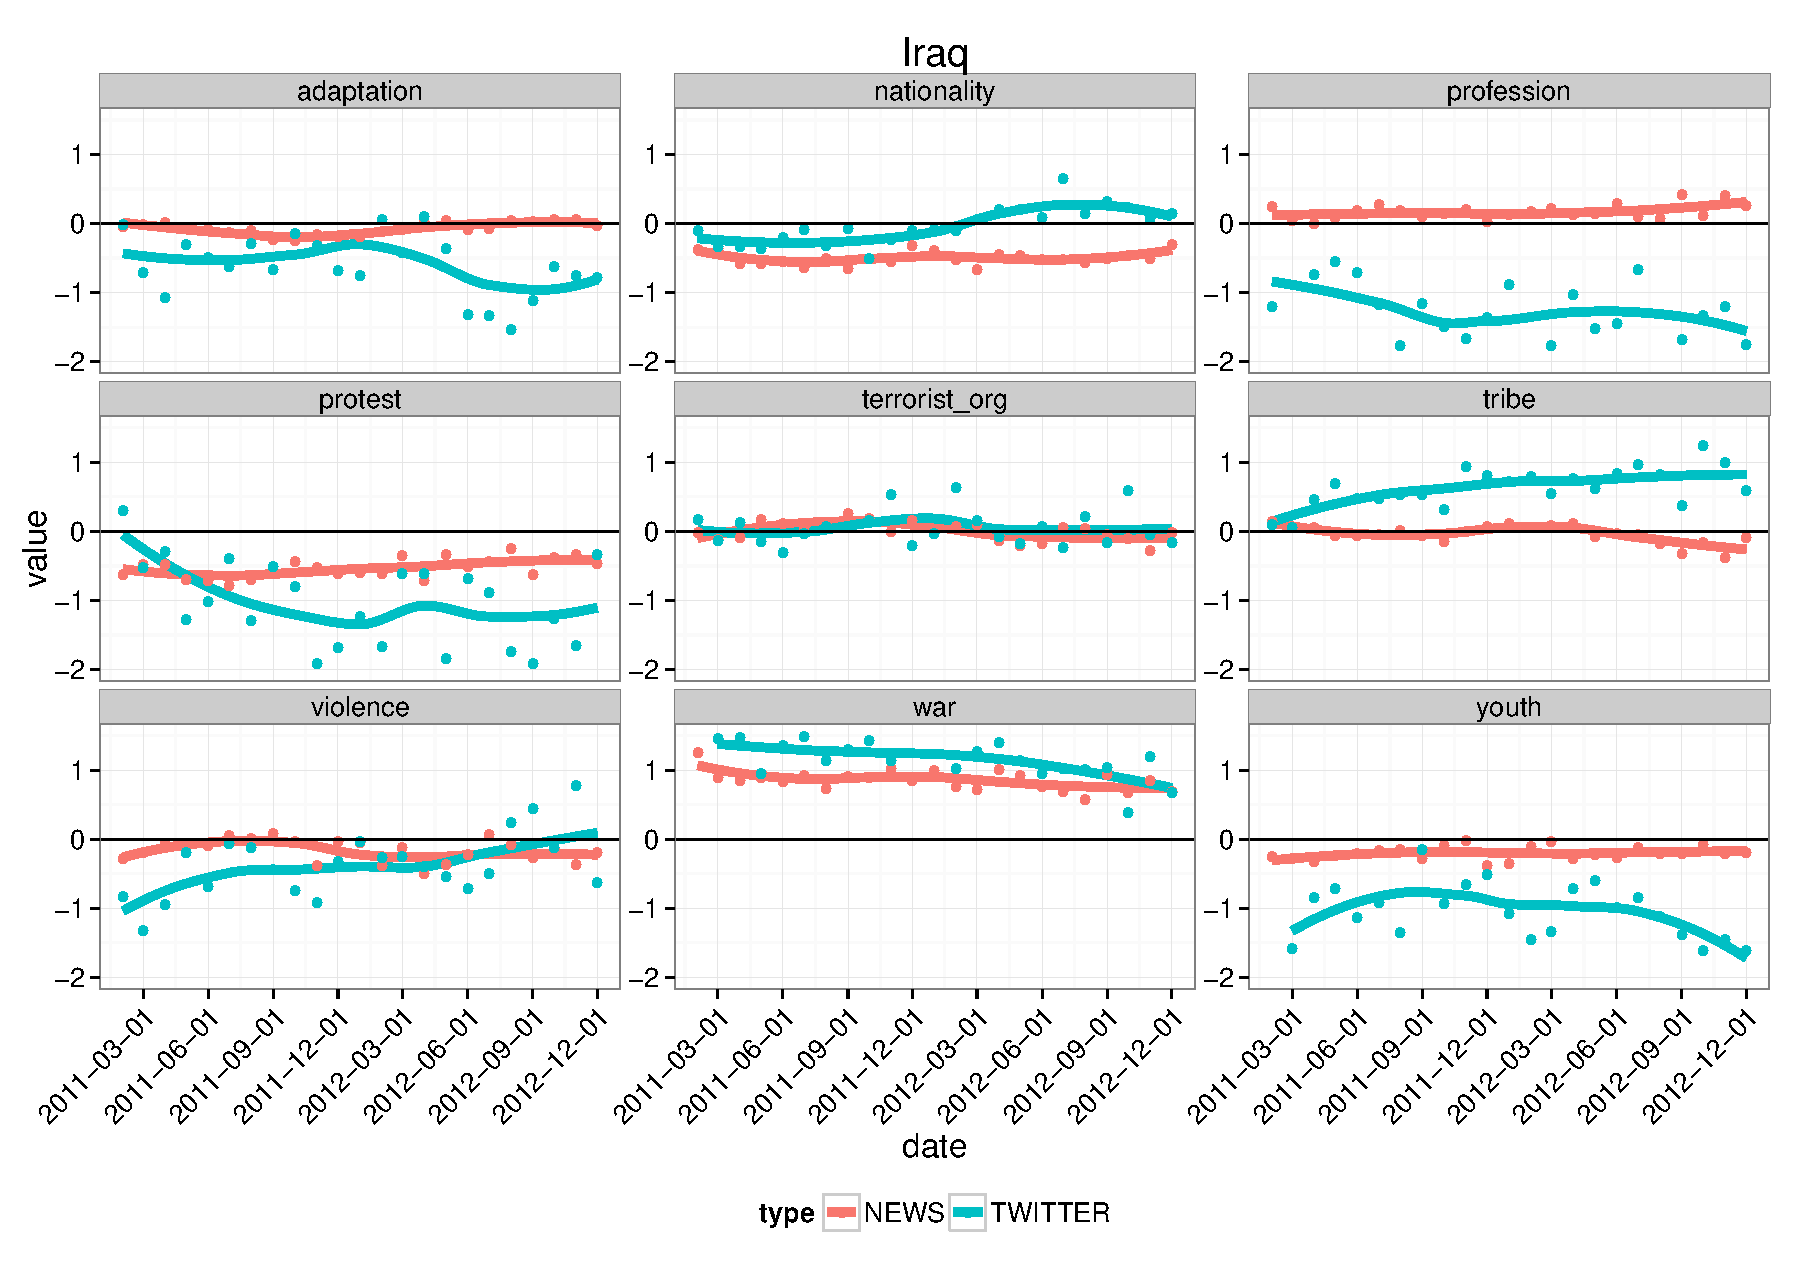
\includegraphics[width=\textwidth]{imgs/iraq.pdf}
%		\caption{Iraq}
%		\label{fig:iraq}
%	\end{figure*}
%	
%	
%	\begin{figure*}
%		\centering
%		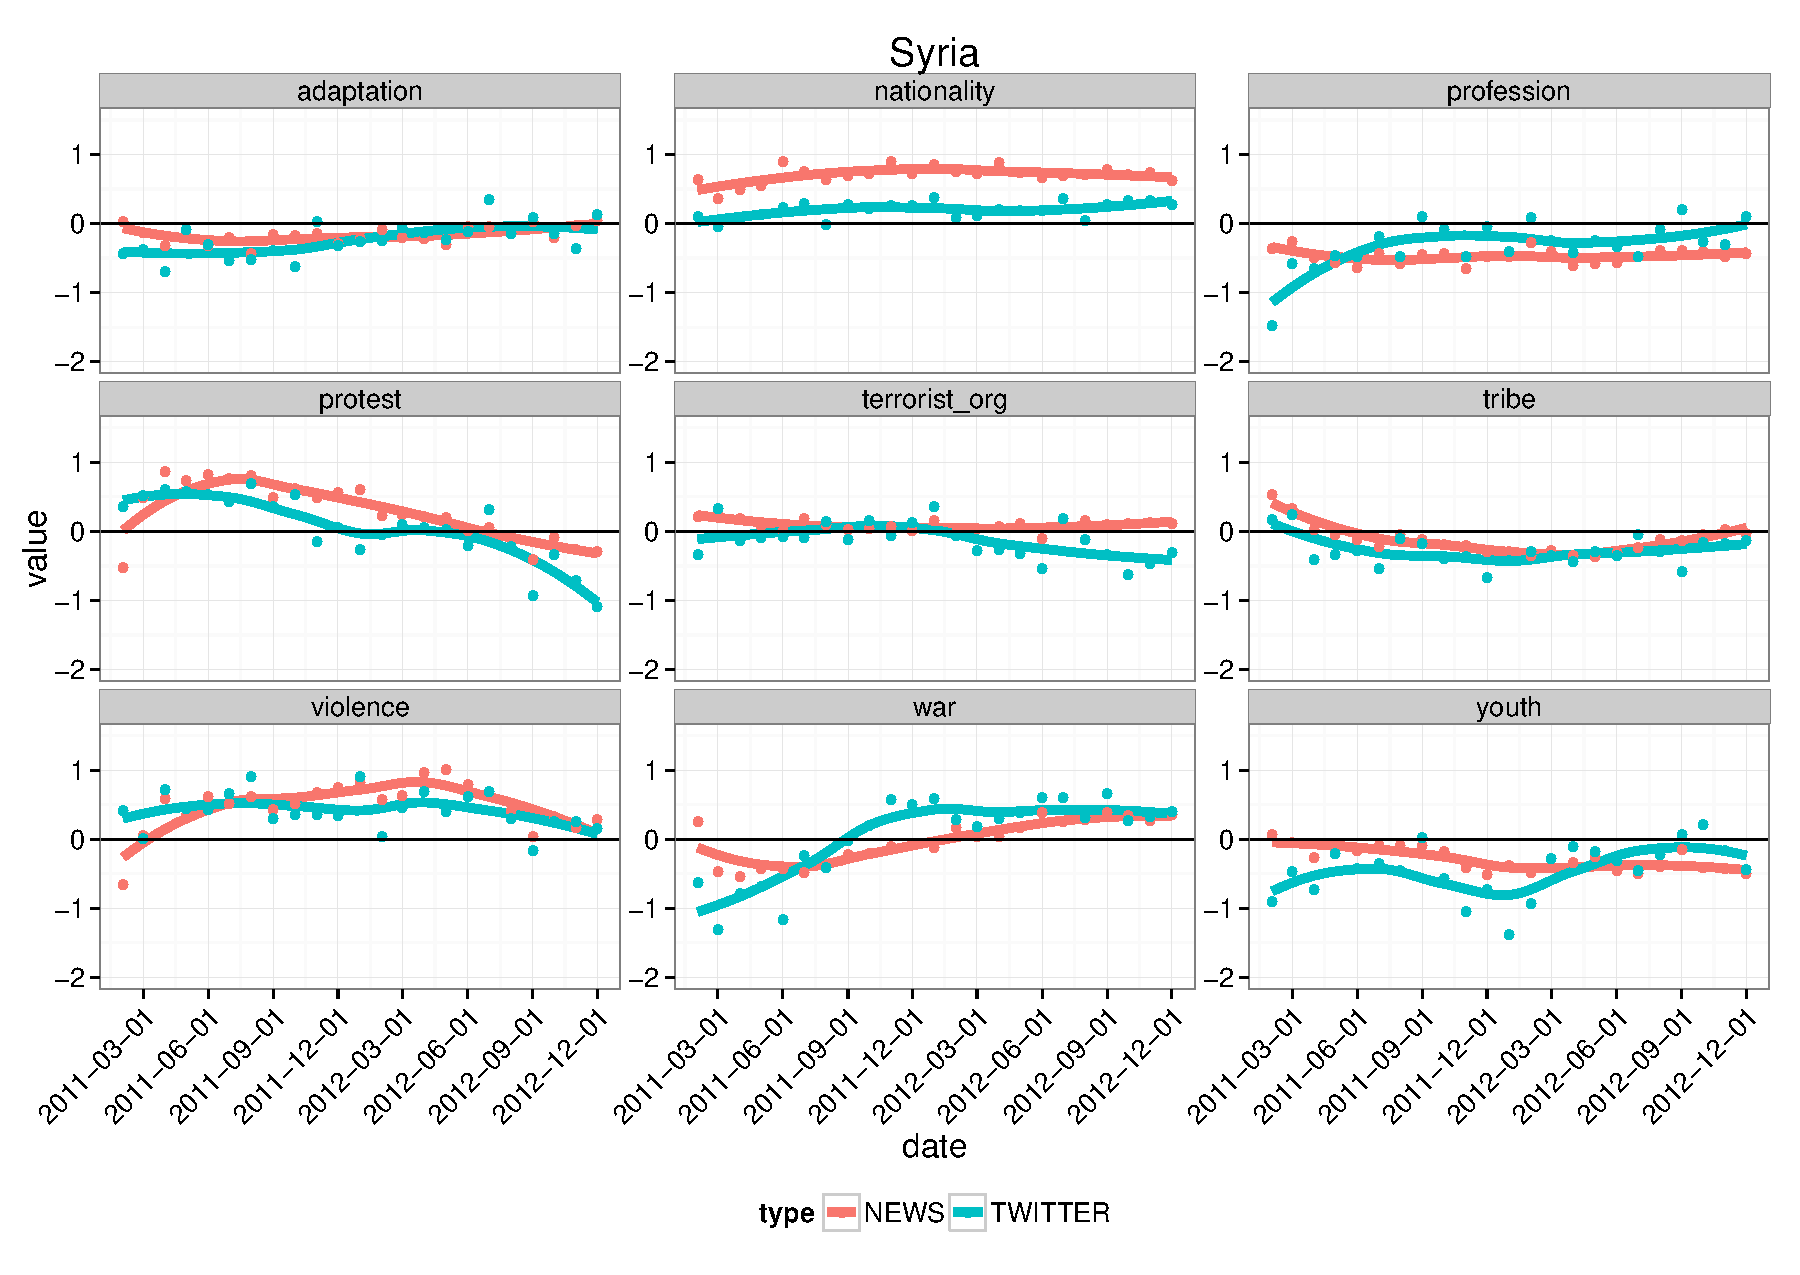
\includegraphics[width=\textwidth]{imgs/syria.pdf}
%		\caption{Syria}
%		\label{fig:syria}
%	\end{figure*}
%	 





